The first construction in the proof of Theorem \ref{thm:3stein4} is a 3--handlebody regular neighbourhood of the 1--skeleton of our Stein complex $S$.
Put $G$ to be the 1--skeleton of $S$ and $A\subset G$ a maximal spanning tree.
We know that $G$ is a graph where, for any vertex $v$ of $G$, $\deg_G v$ is 3 if $v$ is boundary and 4 if it is interior.

We first triangulate the building blocks of Figure \ref{fig:3thickeningblocks}, where each block is depicted as a 3--disc whose boundary is decorated by a graph with blue vertices and red edges.
Our initial triangulations appear in Figure \ref{fig:3thicktri}, where we see triangulated 2--spheres from one perspective.
There are two important properties of these triangulations.
The first is that the red edges appear as triangulated 1--submanifolds (in these basic block they are single edges).
The second is that there are triangulated 2--disc submanifolds about each blue vertex (appearing as single triangles in the basic blocks), and these are regular in the sense that the triangulated edge blocks can be glued to the vertex blocks in such a way that the red edges line up.
The cone on each of these 2--spheres yields initial 3--disc blocks.
Two barycentric subdivisions of these blocks maintain the above properties and deliver a third desirable property: that the triangulated half--tubular neighbourhoods of distinct curves are disjoint.
This means that upon 4--thickening any 3--prism used in the thickening that intersects one thickened curve intersects no other 3--prisms that intersect a different curve.
We take these subdivided triangulations as our \emph{vertex} and \emph{edge blocks}, and the special triangulated red boundary curves as \emph{framing pieces}.

The proof of Theorem \ref{thm:3stein4} is procedural in its creation of handlebodies, and the details for the triangulated case are contained in Algorithm \ref{alg:4handlebody}.
In this section we use the notation laid out in the proof of Theorem \ref{thm:3stein4}, and we take $A\subset G$ to be fixed throughout.

The result of Algorithm \ref{alg:4handlebody} is a 4--handlebody that is a 4--thickening of $U_S(G)$ along with a set of curves in the boundary of that handlebody.
In Algorithm \ref{alg:attachingregions} we find a set of solid torus regions for 2--handle attachment and their associated 0--framing strips as discussed in Theorem \ref{thm:3stein4}.
The curves of Algorithm \ref{alg:4handlebody} are the boundaries of the strips of Algorithm \ref{alg:attachingregions}, and we find the 0--framing curve of the attaching regions based on the type of strip.
When the strip is an annulus, the curve is found as one of the boundary components of the annulus.
When it is a M\"obius strip, there is one boundary component $2\gamma$.
We take $2\gamma$ halfway around its length to one full longitude of $V$, and perform one last positive half twist in order to get an actual 0--framing curve $\gamma$.
To be precise, the half twist is a curve $\gamma$ in the meridian direction of the boundary of $V$ connecting the endpoints of $\frac{1}{2}(2\gamma)$, and the positive direction is the anticlockwise direction determined by the $\II^2$ fibers over the boundary component of $U_S(G)$.
We perform this half twist on the boundary of a part of the solid torus contributed by a vertex block so that we can make more well structured arguments in Section \ref{sub:gleams}.

\begin{algorithm}
	\caption{Building the 4--handlebody of the 1--skeleton of the Stein complex}
	\label{alg:4handlebody}
	\KwData{a Stein complex $S$}
	\KwResult{a triangulated 4--manifold $A_4$ that is the 4--thickening of $U_S(G)$ and a set of embedded framing curves in the boundary of $U_S(G)$}
	\Begin{
		$A_3,C\longleftarrow\emptyset$\;
		\ForEach{vertex $v$ of $A$}{
			add the triangulated vertex block $v_B$ associated to the type of vertex $v$ is in $S$ to $A$\;
			add the framing pieces in the boundary of $v_B$ to $C_A$\;
		}
		\ForEach{edge $e=(u,v)$ of $A$}{
			attach the triangulated edge block $e_B$ associated to the type of edge $e$ is in $S$ over the blocks $u_B$ and $v_B$\;
			add framing pieces in the boundary of $e_B$ to $C_A$\;
			combine the pieces in $C_A$ over identical boundaries\;
		}
		$A_4\longleftarrow$ result of Algorithm \ref{alg:nthickening} with input $A_3$\;
		$C_A\longleftarrow$ the inclusions of $C_A$ into the copies of $A_3$ at $A_3\times\{\pm1\}$ in $A_4$\;
		\ForEach{edge $e=(u,v)$ of $e(G)\setminus e(A)$}{
			$e_B\longleftarrow$ the triangulated edge block associated to the type of edge $e$ is in $S$\;
			$E_B\longleftarrow$ the result of Algorithm \ref{alg:nthickening} with $e_B$\;
			attach $E_B$ over the thickenings $U_B$ and $V_B$ of $u_B$ and $v_B$ in $A_4$ in the unique orientation preserving way\;
			add the framing pieces included into the copies of $e_B$ at $e_B\times\{\pm 1\}$ in $E_B$ to $C_A$\;
			combine the curves in $C_A$ over identical boundaries\;
		}
	}
\end{algorithm}		
		
\begin{algorithm}
	\caption{Finding attaching regions and 0--framing strips for 2--handle attachment}
	\label{alg:attachingregions}
	\KwData{a Stein complex $S$}
	\KwResult{a triangulated 4--manifold $A_4$ that is the 4--thickening of $U_S(G)$, a set of trianglated solid tori $\mathcal{V}$ in the boundary over which we will attach 2--handles, and a set of strips $\mathcal{C}$ in the boundary tori of $\mathcal{V}$ used to determine 0--framings as in the proof of Theorem \ref{thm:3stein4}}
	\Begin{	
		$A_4, C_A\longleftarrow$ result of Algorithm \ref{alg:4handlebody} with input $S$\;
		$\mathcal{V},\mathcal{C}\longleftarrow\emptyset$\;
		\ForEach{curve $c$ of $C_A$}{
			$V\longleftarrow\emptyset$, the solid torus associated with $c$\;
			$C\longleftarrow\emptyset$, the strip in $V$ that determines 0--framing\;
			\ForEach{4--prism $P^4$ in the 4--thickening structure of $A_4$ intersecting $c$ nontrivially}{
				\ForEach{wall $P^3$ of $P^4$}{
					\If{$P^3\cap c$ is nonempty}{
						\ForEach{wall $P^2$ of $P^3$}{
							\If{$P^2\cap c$ contains edges of $c$ \& $P^2$ is not yet in $ C$}{
								add $P^2$ to $C$\;
							}
						}						
						add $P^3$ to $V$\;	
					}
				}
			}
		}
		combine the elements of $V$ over identical boundaries\;
		add $V$ to $\mathcal{V}$\;
		combine the elements of $C$ over identical boundaries\;
		add $C$ to $\mathcal{C}$\;
	}
\end{algorithm}

\begin{figure}
	\centering
	\captionsetup{justification=centering}
	\caption{The triangulated blocks used in the 3--thickening of the 1--skeleton of the Stein complex}
	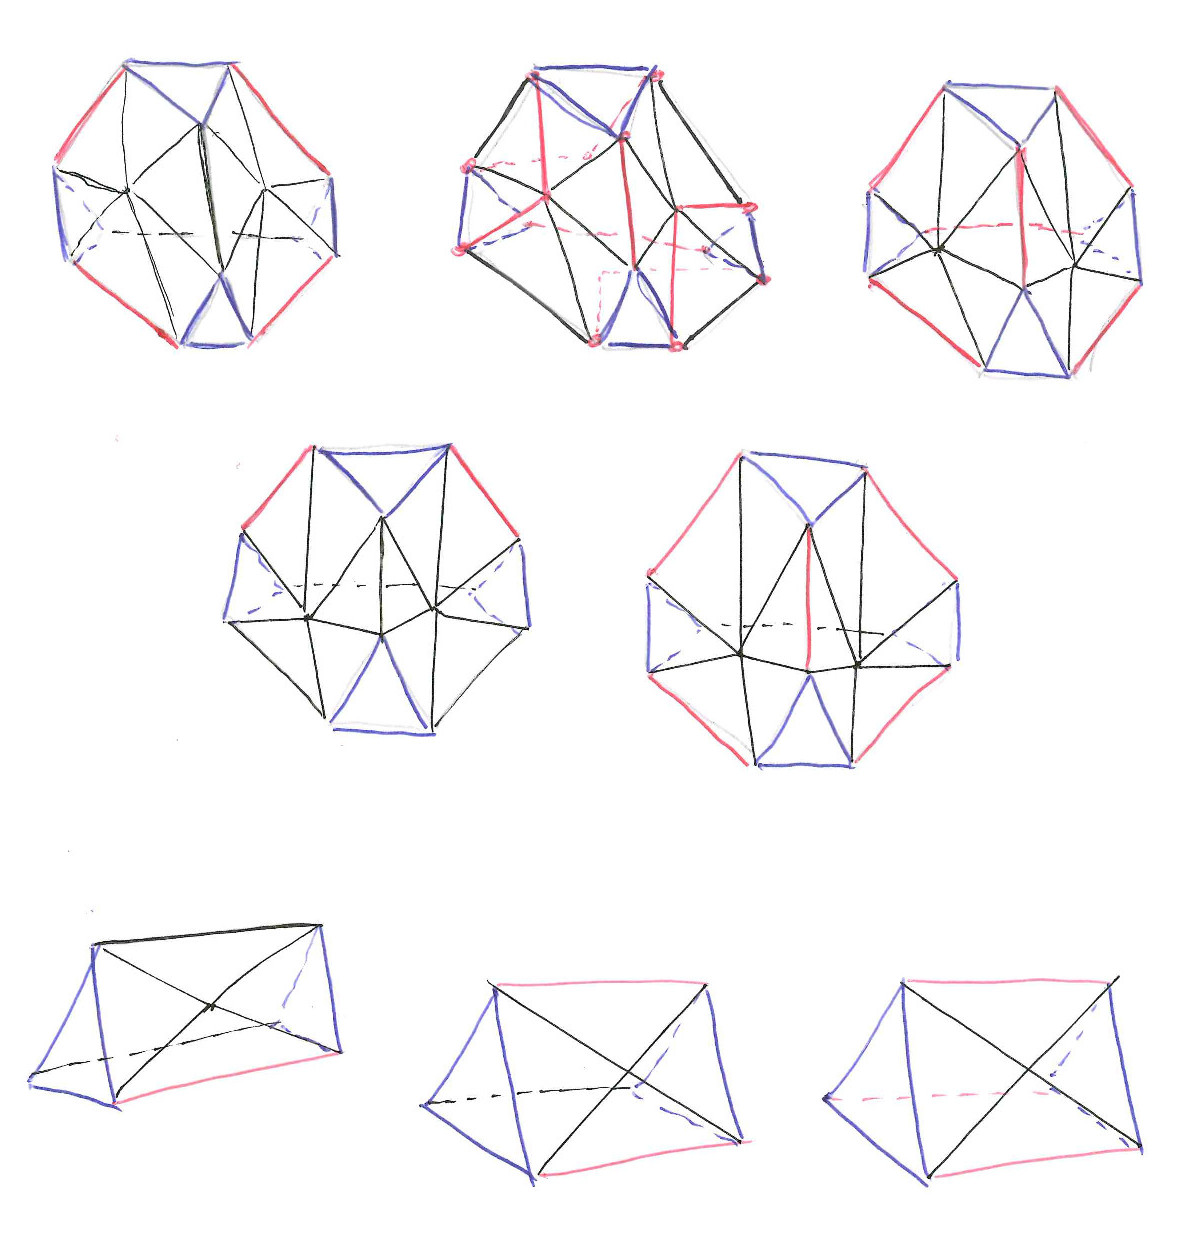
\includegraphics[width=5in]{figures/3thicktri.jpg}
	\label{fig:3thicktri}
\end{figure}